\chapter{多摄像头系统的拍摄时间检测}

\section{本章引言}

对于多摄像头系统来说,控制各个摄像头在特定时刻进行拍摄是其主要的同步方法。在实际的系统应用过程当中,服务器会通过网络发送信号,控制各个摄像头进行拍摄,但是在系统内可能存在多种因素导致摄像头的真实拍摄时间与服务器设定的拍摄时间不符,而这也就导致了多摄像头系统内存在的同步误差。比如服务器发送命令控制各个摄像头在$t_1$时间后进行拍摄,但是服务器程序运行会消耗一定的时间$t_2$,控制命令经网络由服务器传输给各个摄像头,传输过程会消耗一定时间$t_3$。摄像头接收到命令设定自身参数在$t_1$时间后拍摄,而在$t_1$时刻摄像头开始拍摄时,又会消耗掉一定的硬件响应时间$t_4$,因此摄像头真实的拍摄时间并非服务器设定的$t_1$,而是$T = t_2 + t_3 + t_1 + t_4$。并且系统中可能存在的各种延时随机出现,对于各个摄像头来说其延时长短也同样不确定,无法准确进行预测。

\begin{figure}[h] 
  \centering
  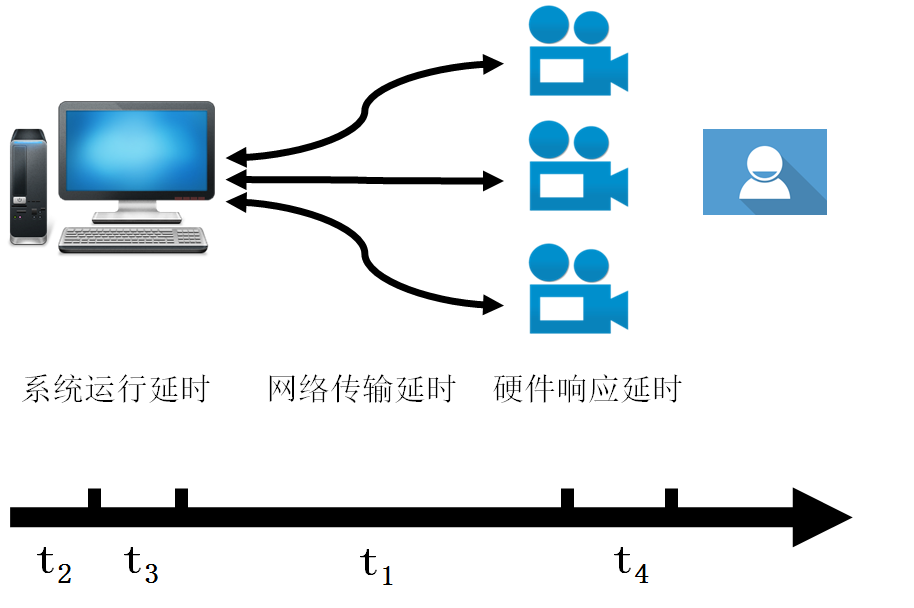
\includegraphics[height=6.5cm, width=8.5cm]{延时}
  \caption{多摄像头系统拍摄过程中可能存在延时}
\end{figure}

因此,对于多摄像头系统来说,为了提高同步精度,并且检验同步效果,就不能仅仅依靠系统内部时钟虽显示的时间进行判断,需要借助外界参考物来检测各个摄像头的拍摄时间。本章提出了一种基于LED点阵的拍摄时间检测方法。该方法利用FPGA控制LED点阵作为检测器,通过设计不同编码方法使点阵显示不同的状态序列。当摄像头拍摄到检测器图像后,对图像进行分析,从而检测出摄像头真实的拍摄时间。该方法通过图像进行检测,排除了系统内部各项误差因素的干扰,并且检测器与摄像头相互分离无需数据通信,同时还适用于多种帧率、曝光时间的摄像头,保证了该方法的普适性。通过对检测器参数的调整可以实现不同精度的检测,且无需调整摄像头参数,使得该方法能够在摄像头正常工作过程中实时进行检测。

\section{拍摄时间检测方法}

采用本方法对摄像头拍摄时间进行检测,主要可分为如下3个步骤:

\textbf{(1)检测器初始化:}该方法的检测器由FPGA控制器和LED点阵两部分组成,分别实现了系统控制和检测信号显示的功能。在初始化阶段,编写控制程序利用FPGA控制LED点阵中各个LED灯的亮灭变化,显示出不同的LED灯组合状态。当每个状态持续一段时间,若干不同状态即可组成状态序列。因此,通过调整FPGA的控制策略,即可控制LED点阵服从一定的编码规律。而根据此规律又可以确定每个LED点阵状态在状态序列当中所处的位置,即可确定每个状态出现的时间。

\textbf{(2)获取检测图像:}设置好检测器后,在需要对拍摄时间进行检测时,将LED点阵置于多摄像头系统的拍摄范围内,控制各个摄像头对其进行拍摄,并将图像保存供分析处理,只需保证拍摄到的图像清晰、完整即可。由于检测器独立于多摄像头系统,相互之间无需进行通信,避免了信号连接、传输、识别等众多操作,有效扩大了该检测方法的适用范围。

\textbf{(3)分析图像计算拍摄时间:}当获得各个摄像头拍摄到的LED点阵图像后,利用图像处理服务器对各副图像进行处理分析。在每幅图像当中提取LED点阵所在位置,并分析点阵当中各个LED灯的亮灭情况,即LED点阵在摄像头拍摄时刻的状态,从而可以根据LED点阵的编码规律确定此状态在序列当中所处的位置,即可以推断摄像头拍摄的时间。多个摄像头之间也可以根据拍摄到的状态的不同确定拍摄时间间隔。

根据在初始化时选择的编码方式的不同,检测出的拍摄时间精度也不尽相同。为了提高该方法的检测精度,要求每个LED点阵状态的持续时间较短,因此要求LED点阵的变化频率较高,对于控制信号的响应速度较快。同时,为了使状态序列足够长,要求LED点阵包含足够多的LED灯,使其能够组合成足够多的不同状态。另外,由FPGA控制LED点阵中各个LED灯期进行变化,因此要求FPGA具有特定接口能够向LED点阵发送控制信号。并且为了在点阵高频率变化时保证足够的时间精度,要求FPGA处理信号和传输信号的时间延迟要尽可能小。对于图像识别服务器来说,为了保证检测的准确性和高精度要求,其对于LED点阵的识别和对于LED灯亮灭状态的判断需要具有更高的准确性。

\section{LED点阵编码方法}

对LED点阵中各个LED灯的亮灭变化情况进行编码,目的是为了使每个由LED灯组成的点阵状态具有唯一性,并且形成特定的状态序列,以便能够对摄像头拍到的状态进行识别,确定该状态在序列中所处的位置,同时还要尽可能提高识别正确率。因此,对于点阵编码方法,要求其具有唯一性、有序性、易识别性。针对以上要求,本文提出了以下4种编码方法,并对其进行了比较。不失一般性,以下采用如图~\ref{mat} 所示的4 × 4的LED点阵对编码方法进行描述。

\begin{figure}[h] 
  \centering
  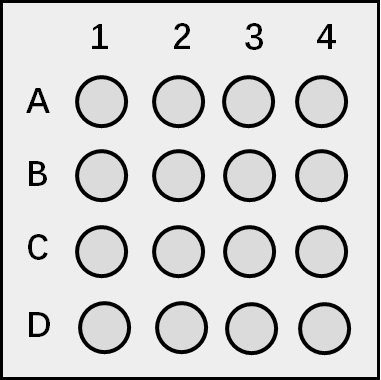
\includegraphics[height=4cm, width=4cm]{点阵}
  \caption{4 × 4的LED点阵}
  \label{mat}
\end{figure}

该点阵共有16个LED灯,依次编号A1、A2、...、B1、B2、...、D4。各个LED灯的亮灭状态相互独立。各个LED灯周期性变化,每个控制周期的持续时间($t_{dur}$)相同。每一个控制周期内,各个LED灯保持亮灭不变,全部LED灯的亮灭状态组成LED点阵在该周期内的状态,全部LED点阵状态组成该编码方法生成的状态序列。各LED灯的亮灭状态和控制周期的时间长短由FPGA控制器进行控制,且控制周期持续时间远远大于LED灯亮灭响应时间和控制信号生成、传输时间。

\subsection{流水编码}

流水编码方法控制LED点阵在一个控制周期内仅有一个LED灯点亮,下一个周期时下一个LED灯点亮,上一周期点亮的LED灯熄灭。各LED灯按照由左至右、由上至下的顺序依次点亮。当最后一个LED灯,即D4灯点亮后,下一周期时D4灯熄灭、A1灯点亮,进行下一循环,如图~\ref{flow}所示:

\begin{figure}[h] 
  \centering
  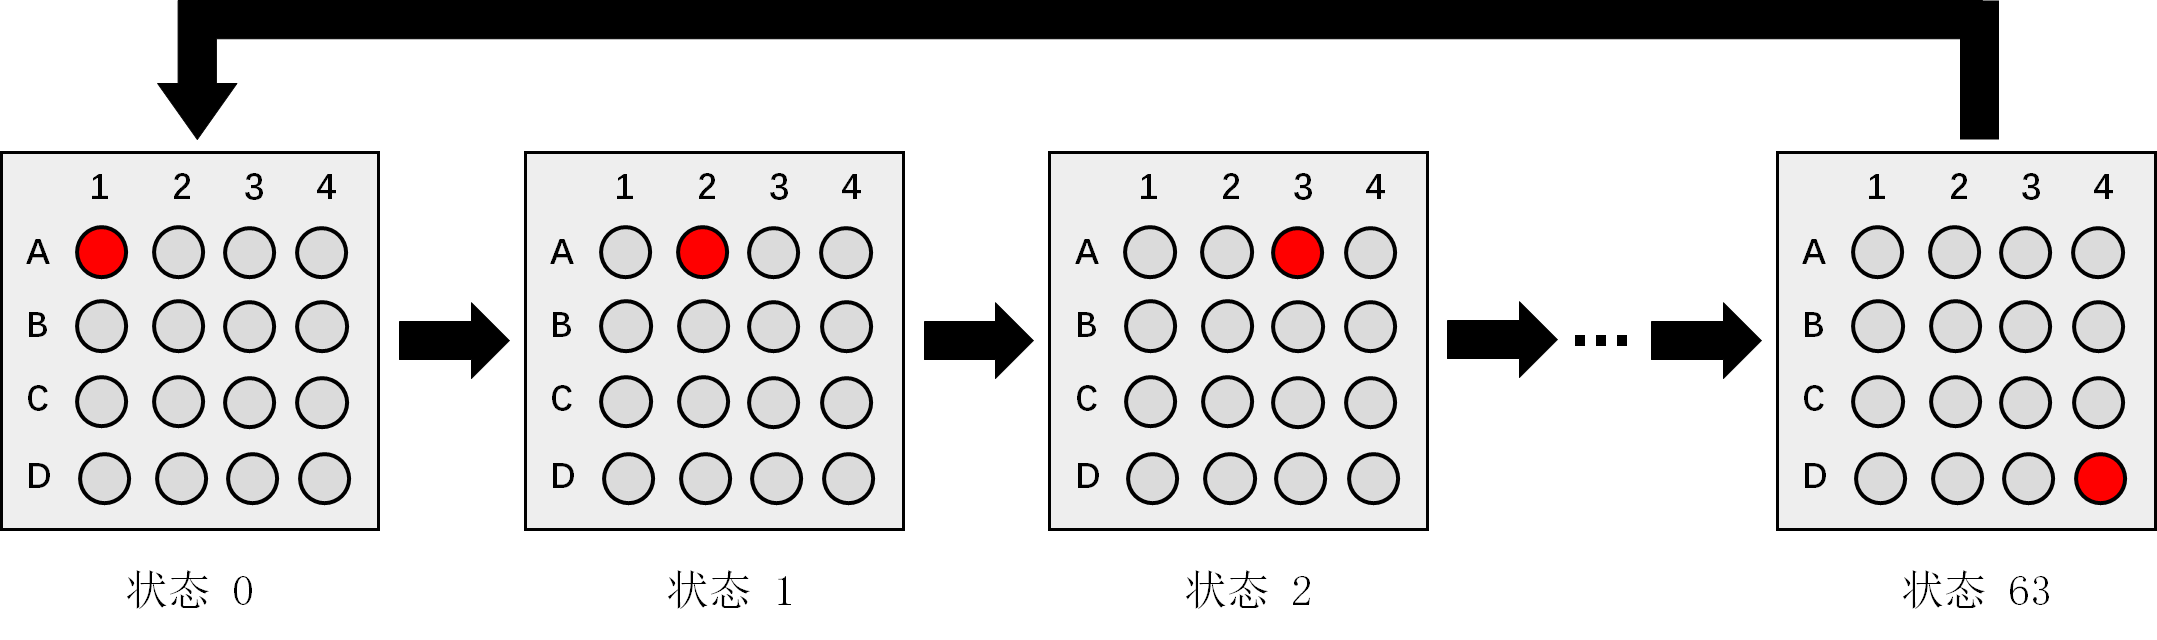
\includegraphics[height=3.6cm, width=12cm]{flow}
  \caption{流水编码的点阵状态序列}
  \label{flow}
\end{figure}

该编码方法实现较为简单,当LED点阵共包含$n$个LED灯,控制周期时间长度为$t_{dur}$时,从第一个LED灯点亮到最后一个LED灯点亮,即一个总的循环周期时间长度($T$)为:

\begin{equation}
T = n * t_{dur}
  \label{flowE}
\end{equation}

当摄像头拍摄到第$k$个状态时,即可以判定其拍摄时刻与LED点阵开始运行时刻之间的时间差为 $k * t_{dur}$。对于两个摄像头分别拍摄到第$k_1$和$k_2$个状态,则这两个摄像头之间的时间差为$(k_1 - k_2) * t_{dur}$。

当摄像头拍摄到某一LED点阵的状态时,可能是在LED点阵保持状态不变的整个控制周期$t_{dur}$中的任意时刻进行拍摄的,因此其检测精度与控制周期的大小有关,最大误差为控制周期时间长度。因此,为了提高检测精度,往往需要控制周期$t_{dur}$较小。同时当LED灯数量较少时,根据公式~\ref{flowE}可知,该编码算法的总循环周期$T$较短。这可能导致在测量过程中使用摄像头拍摄到的不同状态处于不同循环周期内,且无法确定其所属的循环周期,因此最终的测量结果为$x * T + k * t_{dur}$,其中$x$可以取$0, 1, 2...$,总循环周期过小会导致无法确定$x$取值,使得测量结果存在误差。

\subsection{二进制编码}

此编码方法中,将每一个LED灯视为一个二进制数位,LED灯点亮代表1、熄灭代表0,整个LED点阵视为一个16位的二进制数。在每个控制周期内,LED点阵显示一个二进制数,下一个周期时发生变化,按照二进制数变化规律显示下一个二进制数。状态序列如图~\ref{binary}所示:

\begin{figure}[h] 
  \centering
  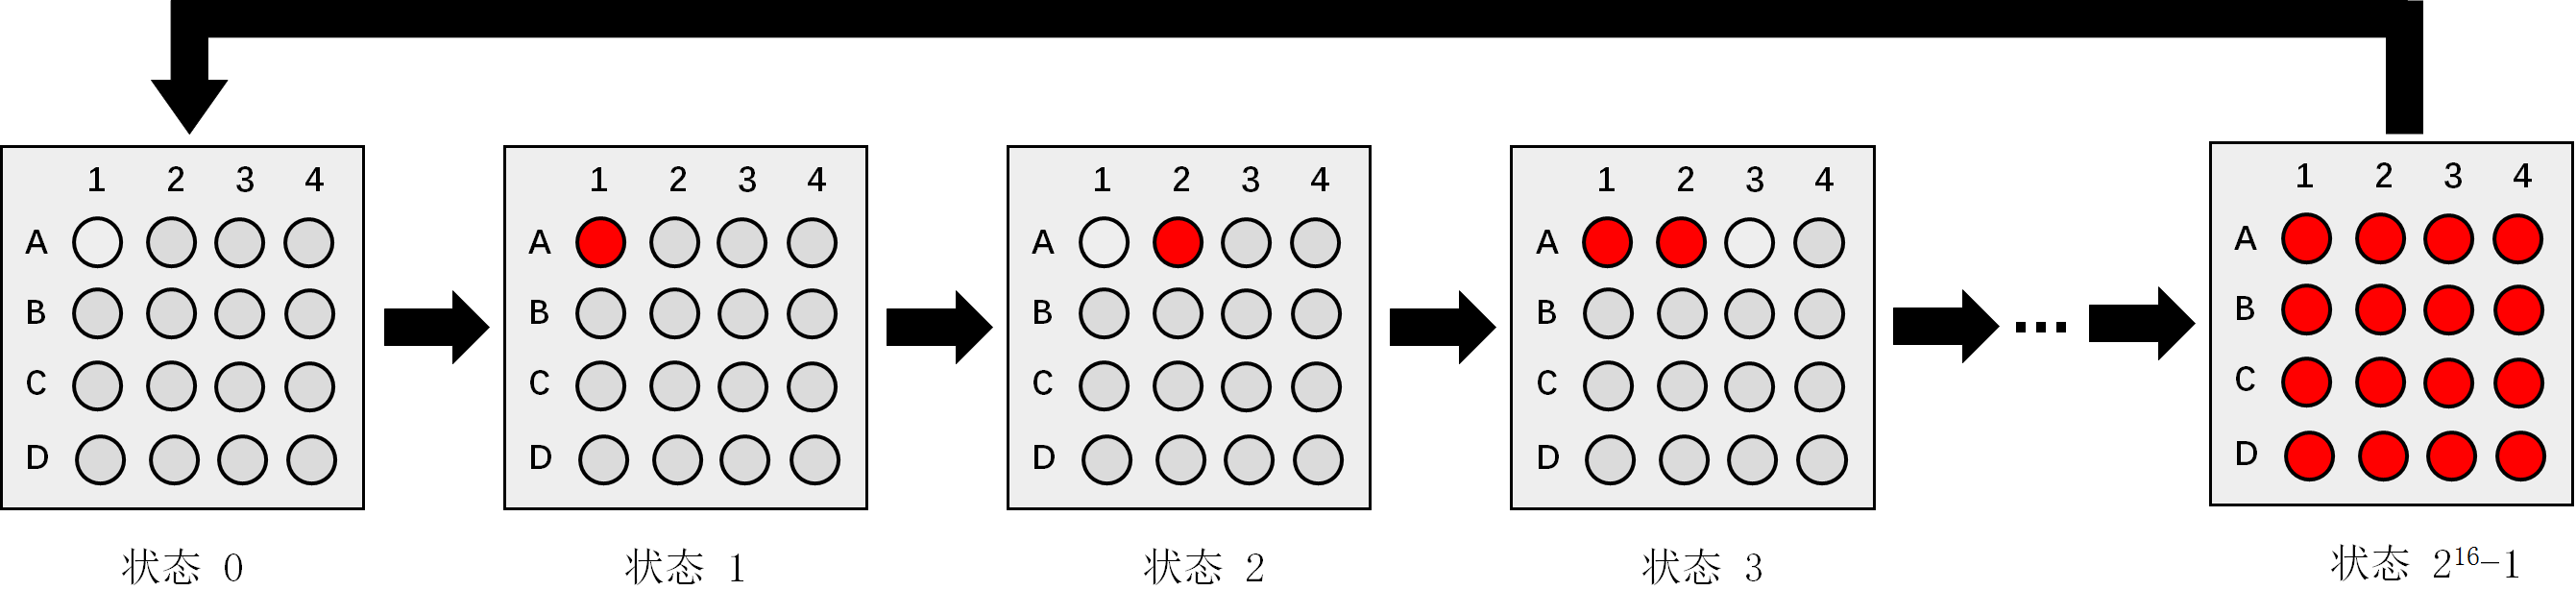
\includegraphics[height=3.6cm, width=14cm]{binary}
  \caption{二进制编码的点阵状态序列}
  \label{binary}
\end{figure}

使用该编码方法,当LED点阵共包含$n$个LED灯时,一个总的循环周期内共有$2^n$个LED点阵状态,则一个总的循环周期的时间长度为:

\begin{equation}
T = 2^n * t_{dur}
\end{equation}

循环周期的时间长度随着LED灯的数量指数增长,因此可以利用较少的LED灯实现较长的循环周期,使得在检测过程中不会出现不同状态属于不同循环周期的情况。二进制编码方法的检测精度同流水编码一样,等于LED点阵的控制周期,即$t_{dur}$。

此方法存在的问题是当摄像机的曝光过程跨越两个或两个以上控制周期时,在一个曝光周期内会拍摄到多个LED点阵状态叠加的图像。由于相邻的若干个状态叠加后的图像不唯一,因此也就无法识别出摄像机拍摄到的图像是由哪几个状态叠加得到的,也就无法判断正确的拍摄时间。例如状态1、状态2叠加和状态2、状态3叠加后得到的图像相同,无法根据叠加图像识别出正确的拍摄时间。

\subsection{格雷码编码}

二进制格雷码(binary gray code)在信号传输领域应用较为广泛,其特点是相邻两个码字中仅有一位发生变化,使得相邻码字的变化最小,能够有效防止数据传输过程当中出现的错误 \cite{mehta1996some, bitner1976efficient},对于四位格雷码和二进制的对应关系如表~\ref{grayT}所示。

\begin{table}[h]
  \centering
  \caption{四位格雷码和二进制} 
  \label{grayT}
  \begin{tabular}{|c|c|c|c|c|c|}\hline
  十进制 & 格雷码 & 二进制 & 十进制 & 格雷码 & 二进制 \\ \hline
  0 & 0000 & 0000 & 8 & 1100 & 1000 \\ \hline
  1 & 0001 & 0001 & 9 & 1101 & 1001 \\ \hline
  2 & 0011 & 0010 & 10 & 1111 & 1010 \\ \hline
  3 & 0010 & 0011 & 11 & 1110 & 1011 \\ \hline
  4 & 0110 & 0100 & 12 & 1010 & 1100 \\ \hline
  5 & 0111 & 0101 & 13 & 1011 & 1101 \\ \hline
  6 & 0101 & 0110 & 14 & 1001 & 1110 \\ \hline
  7 & 0100 & 0111 & 15 & 1000 & 1111 \\ \hline
  \end{tabular}
\end{table}

为了计算两个格雷码之间的差值,可以利用格雷码与二进制码之间转换公式,将格雷码转换为二进制码,然后计算两个二进制码之间的差,即为两个格雷码的差值。对于某个格雷码($g_{n-1}g_{n-2}...g_2g_1g_0$)其对应的二进制数为($b_{n-1}b_{n-2}...b_2b_1b_0$),转换方法如下:

\begin{equation}
\begin{split}
&b_{n-1} = g_{n-1} \\
&b_{i-1} = g_{i-1} \oplus b_{i} \quad i = 1, 2, ..., n-1
\end{split}
  \label{flowE}
\end{equation}

格雷码编码方法同二进制编码方法类似,也是将整个LED点阵视为一个16位的二进制数,按照格雷码的编码规律,在每个控制周期内利用LED灯显示一个格雷码码字。第一个状态为 0000 0000 0000 0000,最后一个状态为 1000 0000 0000 0000,即D4灯点亮。最后一个状态显示结束后,返回至第一个状态,进入下一个循环周期。状态序列如图~\ref{gray}所示:

\begin{figure}[h] 
  \centering
  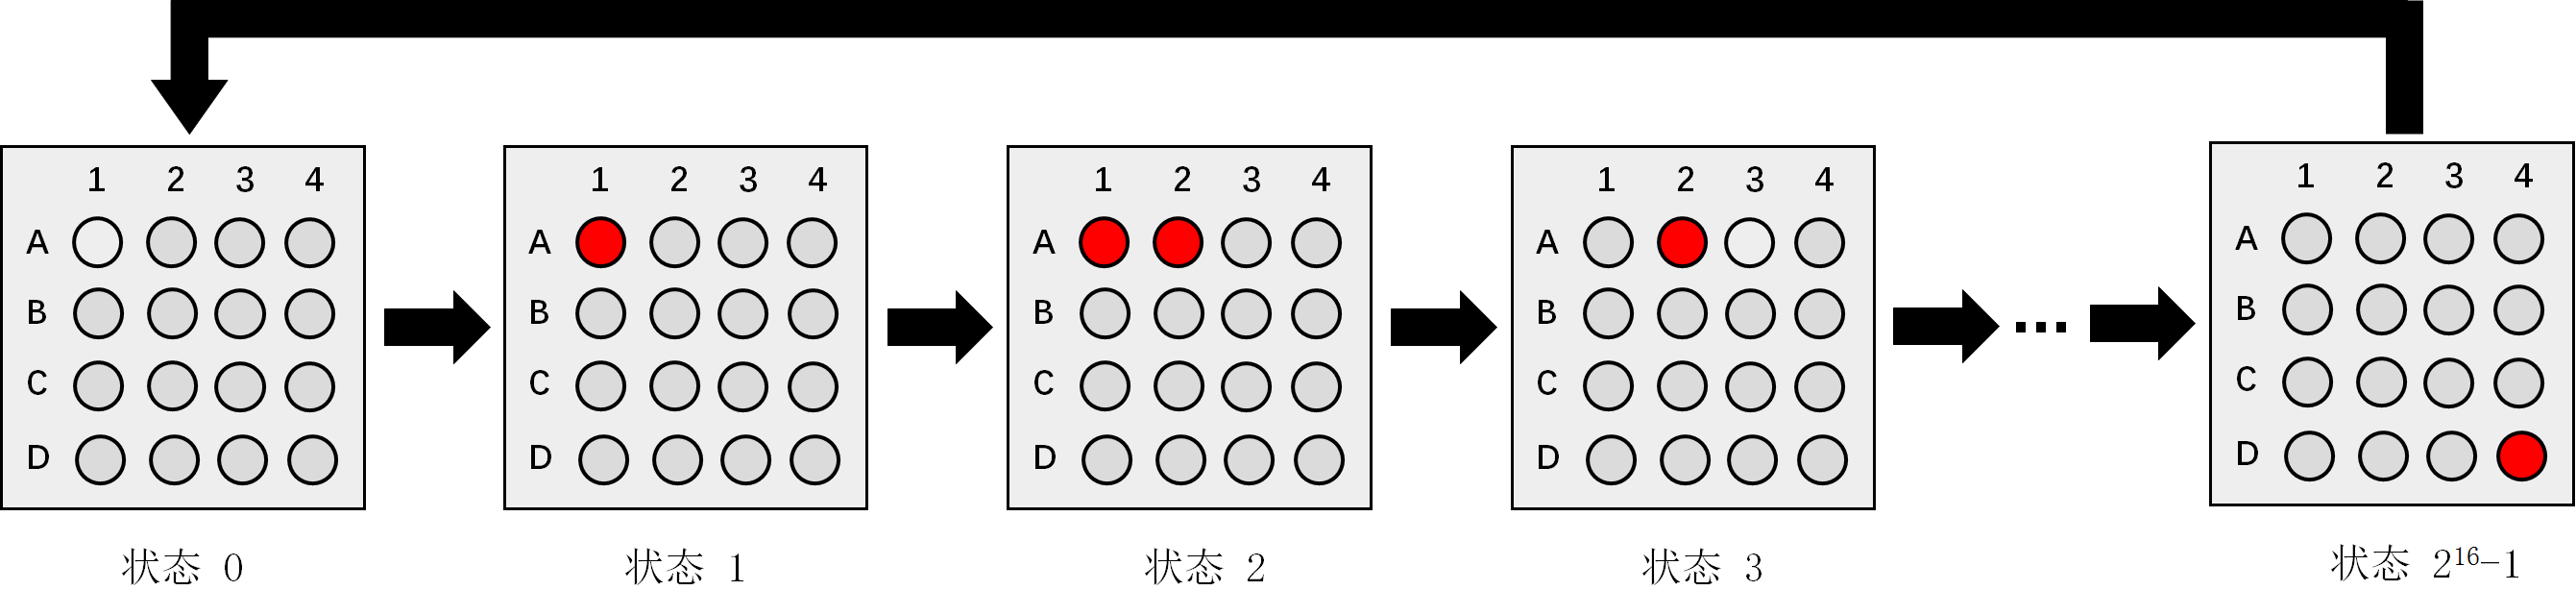
\includegraphics[height=3.6cm, width=14cm]{gray}
  \caption{格雷码编码的点阵状态序列}
  \label{gray}
\end{figure}

使用该编码方法,当LED点阵共包含$n$个LED灯时,一个总的循环周期内共有$2^n$个LED点阵状态,则一个总的循环周期的时间长度为:

\begin{equation}
T = 2^n * t_{dur}
\end{equation}

同二进制编码方法一样,格雷码编码方法也存在状态叠加后的图像不唯一问题。例如状态1、状态2叠加和状态2、状态3叠加后得到的图像相同,无法根据叠加图像识别出正确的拍摄时间。但是,当采用格雷码编码时,如果摄像头曝光时间与控制周期时间相同或小于控制周期时,摄像头将拍摄到一个状态的图像或者是两个状态的叠加图像。根据格雷码特点可知,当一个状态与其相邻状态叠后,只有一位发生变化,因此识别误差相对于二进制编码方法较小。例如,对于4位二进制编码,第3个状态0011与第4个状态0100叠加得到第7个状态0111,与真实状态相差3或4个控制周期。而对于4位格雷码编码,第3个状态0010与第4个状态0110叠加得到第4个状态0110。但是当调整控制周期,使得拍摄图像中有多个状态叠加时,并不能保证只有一位发生变化,仍然会产生较大识别误差。

\subsection{分组叠加编码}

为了解决二进制编码和格雷码编码存在的问题,在格雷码编码的基础上提出分组叠加编码方法。由于在检测过程中拍摄到LED点阵状态叠加是不可避免的,而且状态叠加造成的识别误差是由于叠加状态后得到的码字不唯一所导致,因此可以设计一种编码方式,使得在两种状态叠加时,得到的叠加码字唯一且按规律排列,即使得叠加码字为格雷码。以4位编码为例,状态1、2、3显示的码字分别为0000、0001、0010,则相邻状态叠加得到的叠加码字为0001、0011,满足格雷码编码要求。全部编码序列如图~\ref{over}所示:

\begin{figure}[h] 
  \centering
  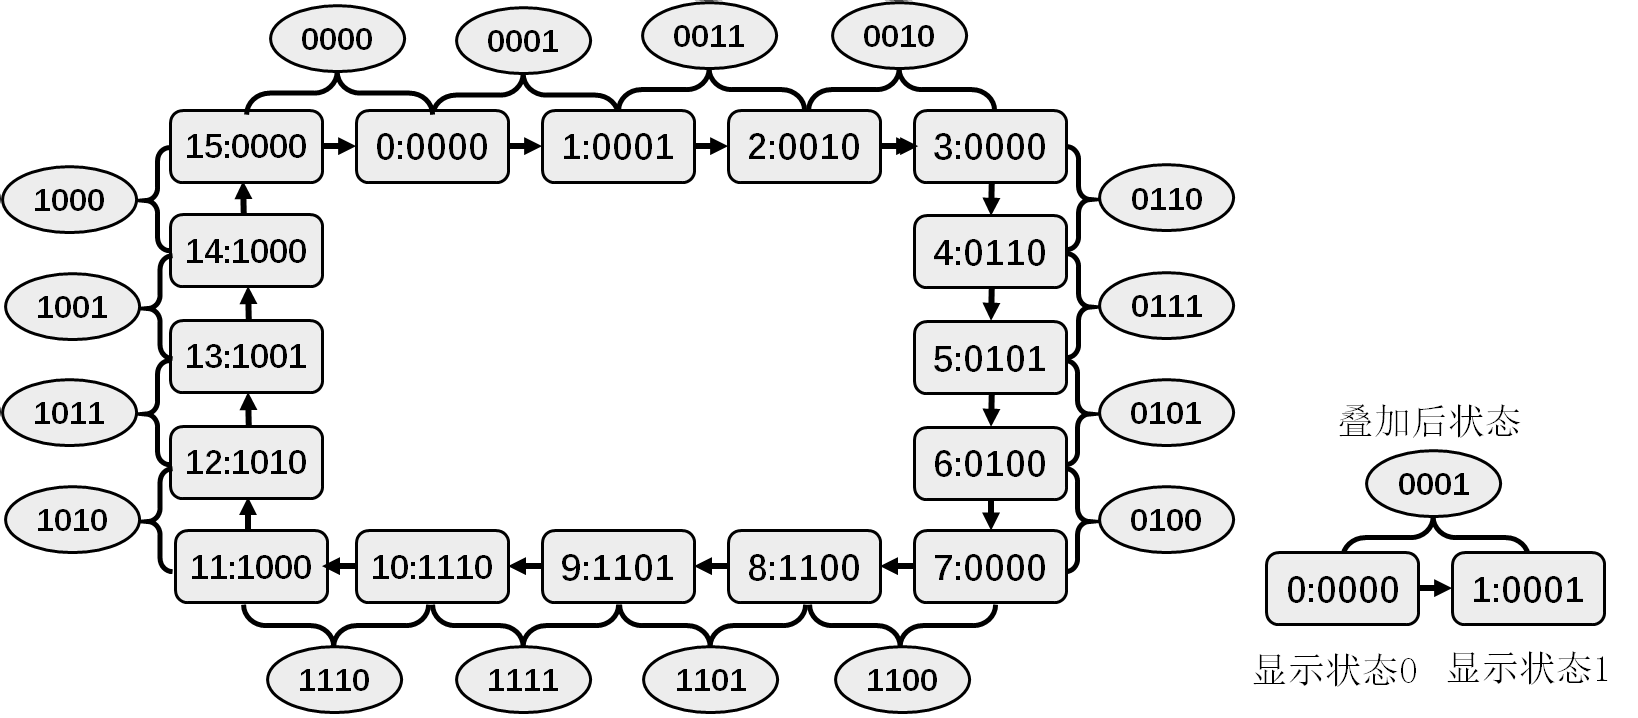
\includegraphics[height=5.5cm, width=14cm]{over}
  \caption{分组叠加编码的码字序列和叠加结果}
  \label{over}
\end{figure}

设定摄像头曝光时间为$k$倍($k$为正整数)控制周期时间长度,则大部分情况下在一个曝光周期内,摄像拍摄到的图像是$k + 1$个LED点阵状态的叠加。仅当曝光开始时间与某一控制周期开始时间相同时,可拍摄到$k$个状态叠加,但此情况出现概率较低。对于一个4 × 4 LED点阵,取$k = 4$,将每行4个LED灯视为一组,共分为4组。每一组分别按照上述编码方法进行编码,显示编号0到15共16个码字。每个码字显示的持续时间为4个控制周期,但是4组LED灯码字分别相差一个控制周期发生变化,这样即可以保证每个控制周期都有一组码字发生变化,又可以保证LED点阵的状态在各个控制周期内不相同。当摄像头对LED点阵进行拍摄时,能够拍摄到$k + 1 = 5$个控制周期的LED点阵状态的叠加图像,此叠加图像内,各组LED灯所显示的码字都发生且仅发生了一次变化,因此4组LED灯的叠加结果分别满足格雷码序列,且拍摄到的叠加图像是唯一的。

当第一组LED灯显示完显示序列内所有16个码字后,如图~\ref{series}所示状态63,为避免与状态0相同进入小循环,使第一组LED灯即将显示的码字序号减1,即显示第14个码字,然后继续按照上述规律进行变化。当第一组LED灯全部循环结束,即显示完状态511后,将第二组显示的码字序号减1继续进行循环。显示序列如图~\ref{series}所示:

\begin{figure}[h] 
  \centering
  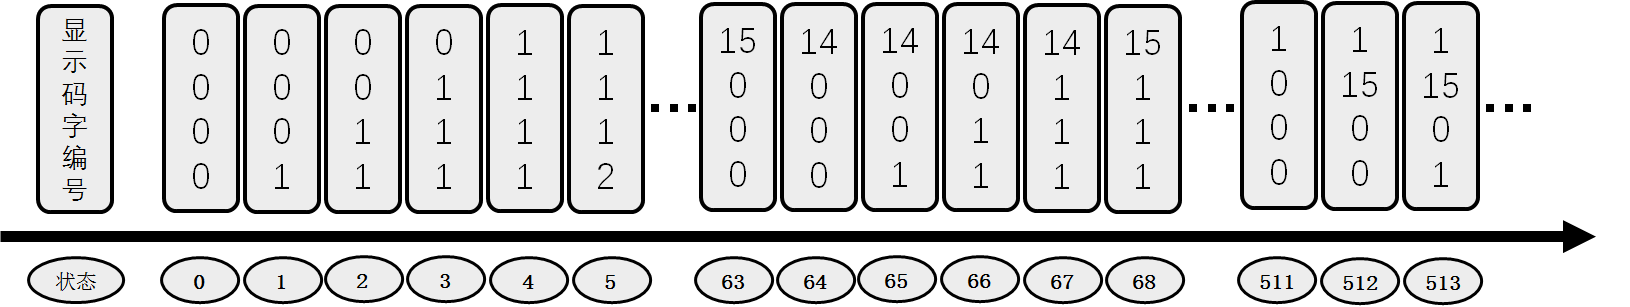
\includegraphics[height=3cm, width=13cm]{series}
  \caption{分组叠加编码的显示序列}
  \label{series}
\end{figure}

具体而言,当摄像头拍摄到状态0至4的叠加图像后,4个组均为第0和第1个码字叠加,因此得到的叠加码字分别为0001、0001、0001、0001。当拍摄到状态1值5时,得到的叠加码字分别为0001、0001、0001、0011。每次拍摄都能得到不同的叠加状态。通过叠加码字可以确定是哪两个显示码字叠加得到,就可以确定摄像头拍摄到的是哪五个状态叠加,从而可以判断摄像头拍摄的开始时刻位于哪个状态内,但是无法判断开始时刻在这个状态内的准确位置。因此检测精度为该状态的持续时间,即控制周期时间长度$t_{dur}$,即曝光时间的四分之一。该编码方法的检测精度($A$)与摄像头曝光时间$t_{exp}$满足如下关系:

\begin{equation}
A = t_{dur} = t_{exp} / k
\end{equation}

则为了提高检测精度,可以降低曝光时间或者增大分组数量。但是一般情况下曝光时间不能过低,因此需要分组数量k较大,也就需要LED点阵中LED灯数量较多。

该方法存在的最大问题在于可操作性欠缺。由于要求各组内相邻两个显示状态叠加而成的叠加状态满足格雷码编码要求,显示状态序列的选取并不存在一定规律。上文示例当中每组包含4个LED灯,而当每组内LED灯数量发生变化时,显示序列同样需要发生变化,且不能保证一定存在满足条件的序列。因此在实际应用当中,该编码方法可操作性较低。

\subsection{进位流水编码}

此方法综合流水编码和分组叠加编码。对于4 × 4 LED点阵,将点阵分为4组,每行1组,每组等级依次升高。每组内各LED灯按照流水编码方法依次点亮。对于等级最低组,即第一组,每个控制周期熄灭当前点亮的LED灯,点亮下一个LED灯。组内最后一个LED灯熄灭后,第一个LED灯点亮,依次循环。对于其他等级组,只有当其低等级组的最后一个LED灯熄灭,发送进位信号给该等级组,该组内才会发生LED灯亮灭变化,熄灭当前点亮的LED灯,点亮下一个LED灯,如图~\ref{composite}所示:

\begin{figure}[h] 
  \centering
  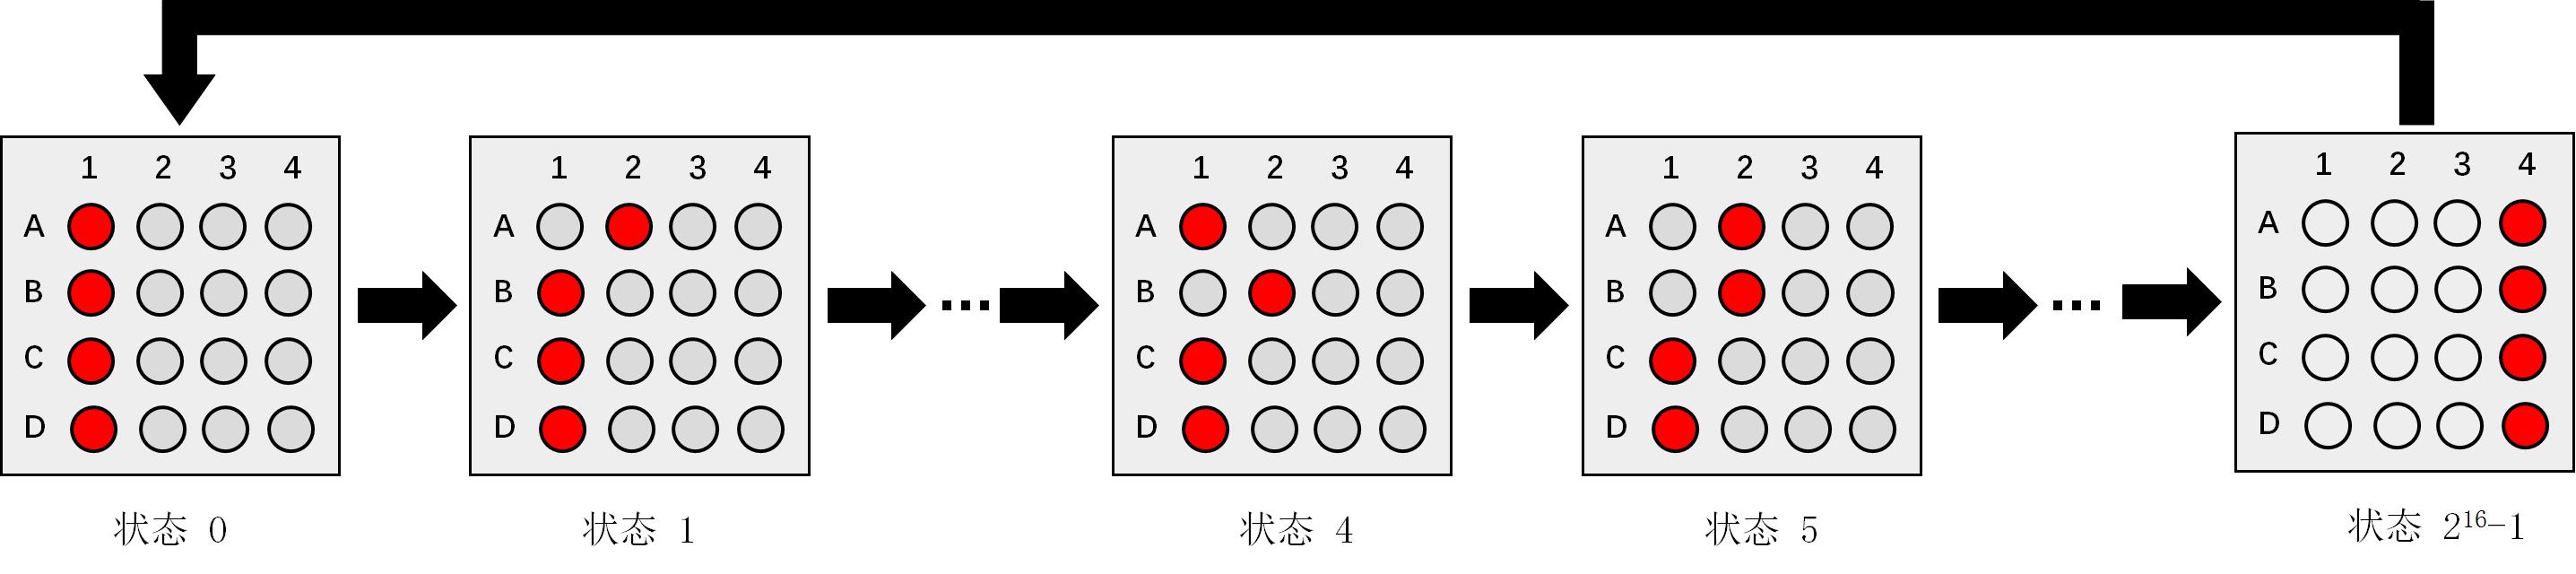
\includegraphics[height=3.5cm, width=14cm]{composite}
  \caption{进位流水编码的点阵状态序列}
  \label{composite}
\end{figure}

假设控制周期的时间长度为$t_{dur}$,将LED点阵分为k组,每组包含$n_i(i = 0, 1, 2, ..., k-1)$个LED灯,每组内各个LED灯亮灭变化的周期长度为$t_i$。最低等级组的变化周期与控制周期时间相同,即$t_1 = t_{dur}$。因为只有当第一组内所有LED灯循环变化一次后才会向第二组发送进位信号,所以第二等级组的变化周期为$n_1 * t_1$。同理则第$i$组的变化周期为:

\begin{equation}
t_i = t_{dur} * \prod_{j=1}^{i-1} n_j
	\label{4}
\end{equation}

通常情况下,摄像头的曝光时间$t_{exp}$要长于控制周期,因此在摄像头拍摄到的图像内有一个以上的LED灯被点亮。同时,$t_{exp}$要短于最高等级组内所有LED灯变化周期之和$n_k * t_k$,因此在摄像头拍摄到的图像内有一个以上的LED灯是熄灭的。一定可以找到第$i$组,使其满足

\begin{equation}
t_i \le t_{exp} \le n_i * t_i
	\label{5}
\end{equation}

当拍摄到的图像内出现状态叠加时,等级低于$i$的组内所有LED灯均被点亮;第$i$组内部分LED灯被点亮,部分熄灭;等级高于$i$的组内有一个或两个LED灯被点亮。对于等级高于$i$的任一组,当与其相邻的低等级组的最后一个和第一个LED灯被点亮时,说明有进位信号产生,因此该组内有两个灯点亮,否则仅有一个灯点亮。当拍摄到一张满足以上描述的LED点阵图片后,首先找到第一个LED灯非全部点亮的等级组$i$;然后判断第$i$组及等级高于$i$的组内第一个被点亮的LED灯,标记其位置分别为 $P_i, P_i + 1, ..., P_k$。 则摄像头的拍摄时间为:
  
\begin{equation}
T = \sum_{j=i}^k p_j * t_j
	\label{T}
\end{equation}

根据公式~\ref{T} 可知,拍摄时间的检测精度为第$i$组内各个LED灯的变化周期$t_i$。根据公式~\ref{4} 可知为了提高检测精度,可以减小控制周期和低等级组内LED灯的数量。同时公式~\ref{5} 要求$t_{exp} \le n_i * t_i$,,需要同时增加第$i$组内LED灯的数目。因此采用进位流水编码方法进行拍摄时间检测时,可以通过减少控制周期长度和低等级组内LED灯的数量,增加高等级组内LED灯的数量来提高检测精度。

\subsection{编码方法比较}

针对以上4种编码方法,利用包含n个LED灯的矩阵,在控制周期为$t_{dur}$的条件下进行比较,比较结果如表~\ref{comp}所示:

\begin{table}[h]
  \centering
  \caption{编码方法比较结果} 
  \label{comp}
  \begin{tabular}{|c|c|c|c|c|c|}\hline
  十进制 & 格雷码 & 二进制 & 十进制 & 格雷码 & 二进制 \\ \hline
  0 & 0000 & 0000 & 8 & 1100 & 1000 \\ \hline
  1 & 0001 & 0001 & 9 & 1101 & 1001 \\ \hline
  2 & 0011 & 0010 & 10 & 1111 & 1010 \\ \hline
  3 & 0010 & 0011 & 11 & 1110 & 1011 \\ \hline
  4 & 0110 & 0100 & 12 & 1010 & 1100 \\ \hline
  5 & 0111 & 0101 & 13 & 1011 & 1101 \\ \hline
  6 & 0101 & 0110 & 14 & 1001 & 1110 \\ \hline
  7 & 0100 & 0111 & 15 & 1000 & 1111 \\ \hline
  \end{tabular}
\end{table}

通过比较可以看出,流水编码总循环周期过短,需要检测器包含较多LED灯才能满足检测需求;格雷码编码在状态叠加的情况下存在识别误差,无法准确检测拍摄时间,且需要摄像头曝光时间较短;分组格雷码在进行高精度检测时需要摄像头较短的曝光时间或者检测器包含较多LED灯;进位流水编码克服了以上三种方法存在的问题,能够进行高精度检测。

\section{图像检测算法}



\section{本章小结}

